%%%%%%%%%%%%%%%%%%%%%%%%%%%%%%%%%%%%%%%%%
% Programming/Coding Assignment
% LaTeX Template
%
% This template has been downloaded from:
% http://www.latextemplates.com
%
% Original author:
% Ted Pavlic (http://www.tedpavlic.com)
%
% Note:
% The \lipsum[#] commands throughout this template generate dummy text
% to fill the template out. These commands should all be removed when 
% writing assignment content.
%
% This template uses a Perl script as an example snippet of code, most other
% languages are also usable. Configure them in the "CODE INCLUSION 
% CONFIGURATION" section.
%
%%%%%%%%%%%%%%%%%%%%%%%%%%%%%%%%%%%%%%%%%

%----------------------------------------------------------------------------------------
%	PACKAGES AND OTHER DOCUMENT CONFIGURATIONS
%----------------------------------------------------------------------------------------

\documentclass{article}

\usepackage{fancyhdr} % Required for custom headers
\usepackage{lastpage} % Required to determine the last page for the footer
\usepackage{extramarks} % Required for headers and footers
\usepackage[usenames,dvipsnames]{color} % Required for custom colors
\usepackage{graphicx} % Required to insert images
\usepackage{subcaption}
\usepackage{listings} % Required for insertion of code
\usepackage{courier} % Required for the courier font
\usepackage{lipsum} % Used for inserting dummy 'Lorem ipsum' text into the template
\usepackage{amsmath}
\usepackage[space]{grffile}

\newcommand{\nb}{\nonumber}

% Margins
\topmargin=-0.45in
\evensidemargin=0in
\oddsidemargin=0in
\textwidth=6.5in
\textheight=9.0in
\headsep=0.25in

\linespread{1.1} % Line spacing

% Set up the header and footer
\pagestyle{fancy}
\lhead{\hmwkAuthorName} % Top left header
\chead{\hmwkClass\ (\hmwkClassTime): \hmwkTitle} % Top center head
%\rhead{\firstxmark} % Top right header
\lfoot{\lastxmark} % Bottom left footer
\cfoot{} % Bottom center footer
\rfoot{Page\ \thepage\ of\ \protect\pageref{LastPage}} % Bottom right footer
\renewcommand\headrulewidth{0.4pt} % Size of the header rule
\renewcommand\footrulewidth{0.4pt} % Size of the footer rule

\setlength\parindent{0pt} % Removes all indentation from paragraphs

%----------------------------------------------------------------------------------------
%	CODE INCLUSION CONFIGURATION
%----------------------------------------------------------------------------------------

\definecolor{MyDarkGreen}{rgb}{0.0,0.4,0.0} % This is the color used for comments
\lstloadlanguages{Perl} % Load Perl syntax for listings, for a list of other languages supported see: ftp://ftp.tex.ac.uk/tex-archive/macros/latex/contrib/listings/listings.pdf
\lstset{language=Perl, % Use Perl in this example
        frame=single, % Single frame around code
        basicstyle=\small\ttfamily, % Use small true type font
        keywordstyle=[1]\color{Blue}\bf, % Perl functions bold and blue
        keywordstyle=[2]\color{Purple}, % Perl function arguments purple
        keywordstyle=[3]\color{Blue}\underbar, % Custom functions underlined and blue
        identifierstyle=, % Nothing special about identifiers                                         
        commentstyle=\usefont{T1}{pcr}{m}{sl}\color{MyDarkGreen}\small, % Comments small dark green courier font
        stringstyle=\color{Purple}, % Strings are purple
        showstringspaces=false, % Don't put marks in string spaces
        tabsize=5, % 5 spaces per tab
        %
        % Put standard Perl functions not included in the default language here
        morekeywords={rand},
        %
        % Put Perl function parameters here
        morekeywords=[2]{on, off, interp},
        %
        % Put user defined functions here
        morekeywords=[3]{test},
       	%
        morecomment=[l][\color{Blue}]{...}, % Line continuation (...) like blue comment
        numbers=left, % Line numbers on left
        firstnumber=1, % Line numbers start with line 1
        numberstyle=\tiny\color{Blue}, % Line numbers are blue and small
        stepnumber=5 % Line numbers go in steps of 5
}

% Creates a new command to include a perl script, the first parameter is the filename of the script (without .pl), the second parameter is the caption
\newcommand{\perlscript}[2]{
\begin{itemize}
\item[]\lstinputlisting[caption=#2,label=#1]{#1.pl}
\end{itemize}
}

%----------------------------------------------------------------------------------------
%	DOCUMENT STRUCTURE COMMANDS
%	Skip this unless you know what you're doing
%----------------------------------------------------------------------------------------

% Header and footer for when a page split occurs within a problem environment
\newcommand{\enterProblemHeader}[1]{
%\nobreak\extramarks{#1}{#1 continued on next page\ldots}\nobreak
%\nobreak\extramarks{#1 (continued)}{#1 continued on next page\ldots}\nobreak
}

% Header and footer for when a page split occurs between problem environments
\newcommand{\exitProblemHeader}[1]{
%\nobreak\extramarks{#1 (continued)}{#1 continued on next page\ldots}\nobreak
%\nobreak\extramarks{#1}{}\nobreak
}

\setcounter{secnumdepth}{0} % Removes default section numbers
\newcounter{homeworkProblemCounter} % Creates a counter to keep track of the number of problems
\setcounter{homeworkProblemCounter}{-1}

\newcommand{\homeworkProblemName}{}
\newenvironment{homeworkProblem}[1][Problem \arabic{homeworkProblemCounter}]{ % Makes a new environment called homeworkProblem which takes 1 argument (custom name) but the default is "Problem #"
\stepcounter{homeworkProblemCounter} % Increase counter for number of problems
\renewcommand{\homeworkProblemName}{#1} % Assign \homeworkProblemName the name of the problem
\section{\homeworkProblemName} % Make a section in the document with the custom problem count
\enterProblemHeader{\homeworkProblemName} % Header and footer within the environment
}{
\exitProblemHeader{\homeworkProblemName} % Header and footer after the environment
}

\newcommand{\problemAnswer}[1]{ % Defines the problem answer command with the content as the only argument
\noindent\framebox[\columnwidth][c]{\begin{minipage}{0.98\columnwidth}#1\end{minipage}} % Makes the box around the problem answer and puts the content inside
}

\newcommand{\homeworkSectionName}{}
\newenvironment{homeworkSection}[1]{ % New environment for sections within homework problems, takes 1 argument - the name of the section
\renewcommand{\homeworkSectionName}{#1} % Assign \homeworkSectionName to the name of the section from the environment argument
\subsection{\homeworkSectionName} % Make a subsection with the custom name of the subsection
\enterProblemHeader{\homeworkProblemName\ [\homeworkSectionName]} % Header and footer within the environment
}{
\enterProblemHeader{\homeworkProblemName} % Header and footer after the environment
}

%----------------------------------------------------------------------------------------
%	NAME AND CLASS SECTION
%----------------------------------------------------------------------------------------

\newcommand{\hmwkTitle}{Assignment\ $1$} % Assignment title
\newcommand{\hmwkDueDate}{Monday,\ January\ 29,\ 2018} % Due date
\newcommand{\hmwkClass}{CSC411} % Course/class
\newcommand{\hmwkClassTime}{L2001} % Class/lecture time
\newcommand{\hmwkAuthorName}{Weixin Liu} % Your name

%----------------------------------------------------------------------------------------
%	TITLE PAGE
%----------------------------------------------------------------------------------------

\title{
\vspace{2in}
\textmd{\textbf{\hmwkClass:\ \hmwkTitle}}\\
\normalsize\vspace{0.1in}\small{Due\ on\ \hmwkDueDate}\\
\vspace{0.1in}
\vspace{3in}
}

\author{\textbf{\hmwkAuthorName}}
%\date{} % Insert date here if you want it to appear below your name

%----------------------------------------------------------------------------------------

\begin{document}

\maketitle
\clearpage

\section*{Notes:}
All the figures used in below can be obtained from the file faces.py. The cropped images are updated to MarkUs as zipfile $cropped\_images$. In order to get faces.py work:
\begin{itemize}
\item Extract the zip file into the directory of which faces.py is located.
\item Or directly download and process the images by uncomment $part1()$ in main block. And place textfile $facescrub\_actors.txt$ and $facescrub\_actresses.txt$ in the directory of which faces.py is located.
\end{itemize}
In order to reproduce the faces.pdf, the images 6a and 6b in the zipfile $part6_latex_images$ should be extracted into the the directory of which faces.py is located. After uncomment $part1()$ and running the faces.py, faces.tex (should be placed in the same directory as which faces.py is at) should be able to  re-generate the faces.pdf.
\clearpage
%----------------------------------------------------------------------------------------
%	PROBLEM 0
%----------------------------------------------------------------------------------------

% To have just one problem per page, simply put a \clearpage after each problem

\begin{homeworkProblem}

\noindent \textit{Brief View of dataset and how to download and process them}

The dataset used in the project is a subset of FaceScrub dataset. (http://vintage.winklerbros.net/facescrub.html). This dataset is provided in form of two text files: facescrub\_actors.txt and facescrub\_actresses.txt. They contain the information of male actors and female actors respectively. Every line in the text file contains all the information of one particular image. The following line is a example line:\\

Lorraine Bracco	20815	9613	http://upload.wikimedia.org/wikipedia/commons/1/1b/Lorraine\_Bracco\_HS\_Yea\\ rbook.jpeg	22,62,135,175	d920e0af8b560d8d9df41baa422314abf24a8c729ed6bab9324e8e15f3e4d6b2\\

"Lorraine Bracco" is the actor's name. "http://upload.wikimedia.org/wikipedia/commons/1/1b/Lorraine\_Br\\ acco\_HS\_Yearbook.jpeg" is a URL where the image can be download from. "22,62,135,175" is the bounding box of the face, which is given in such format: $x_{1}$, $y_{1}$, $x_{2}$, $y_{2}$ where ($x_{1}$, $y_{1}$) is the coordinate of the upper left corner of the bounding box and ($x_{2}$, $y_{2}$) is the coordinate of the lower right corner. \\

The images can be either gray-scale image or color image and may have various sizes. For this project, we need to crop out the images of the faces given the coordinates of the bounding boxes, convert them to grayscale if the image is color, and then, resize them to 32$\times$32. Note that some URLs were dead at the time when downloading them.\\

The code for downloading and processing images is pasted below. The code will first download according to two text files and store the original images into the sub-folders under the directory of which the python file is located. The sub-folders are facescrub\_actors\_cropped and  facescrub\_actresses\_cropped. Then it will process the downloaded images in the foregoing fashion and stores them in other two sub-folders: facescrub\_actors\_cropped and facescrub\_actresses\_cropped. The code is defined as a function. To download and process images, simply call function $part1()$. Note: the variable $dirpath$ is pre-defined in the main block, and it is set to the directory of which the python file is located. \\

\begin{lstlisting}
def rgb2gray(rgb):
    '''Return the grayscale version of the RGB image rgb as a 2D numpy array
    whose range is 0..1
    Arguments:
    rgb -- an RGB image, represented as a numpy array of size n x m x 3. The
    range of the values is 0..255
    '''
    r, g, b = rgb[:, :, 0], rgb[:, :, 1], rgb[:, :, 2]
    gray = 0.2989 * r + 0.5870 * g + 0.1140 * b
    return gray / 255.

def timeout(func, args=(), kwargs={}, timeout_duration=1, default=None):
    '''From:
    http://code.activestate.com/recipes/473878-timeout-function-using-threading/'''
    import threading
    class InterruptableThread(threading.Thread):
        def __init__(self):
            threading.Thread.__init__(self)
            self.result = None

        def run(self):
            try:
                self.result = func(*args, **kwargs)
            except:
                self.result = default

    it = InterruptableThread()
    it.start()
    it.join(timeout_duration)
    if it.isAlive():
        return False
    else:
        return it.result

def part1():
    for act_type in ['actors', 'actresses']:
        faces_subset = dirpath + "/facescrub_" + act_type + ".txt"
        uncropped_path = dirpath + "/facescrub_" + act_type + "_uncropped/"
        cropped_path = dirpath + "/facescrub_" + act_type + "_cropped/"
        if os.path.isdir(uncropped_path):
            os.unlink(uncropped_path)
        else:
            os.makedirs(uncropped_path)

        if os.path.isdir(cropped_path):
            os.unlink(cropped_path)
        else:
            os.makedirs(cropped_path)

        testfile = urllib.URLopener()

        act = list(set([a.split("\t")[0] for a in open(faces_subset).readlines()]))

        # Note: you need to create the uncropped folder first in order
        # for this to work

        for a in act:
            # name = a.split()[1].lower()
            name = a
            i = 0
            for line in open(faces_subset):
                if a in line:
                    filename = name + str(i) + '.' + line.split()[4].split('.')[-1]
                    # A version without timeout (uncomment in case you need to
                    # unsupress exceptions, which timeout() does)
                    # testfile.retrieve(line.split()[4], "uncropped/"+filename)
                    # timeout is used to stop downloading images which take
                    # too long to download
                    timeout(testfile.retrieve, (line.split()[4],\
                     uncropped_path + filename), {}, 5)
                    if not os.path.isfile(uncropped_path + filename):
                        continue

                    try:
                        uncropped = imread(uncropped_path + filename)
                        crop_coor = line.split("\t")[4].split(",")
                        if (uncropped.ndim) == 3:
                            cropped = uncropped[int(crop_coor[1]):int(crop_coor[3]),\
                                      int(crop_coor[0]):int(crop_coor[2]), :]
                            resized = imresize(cropped, (32, 32))
                            grayed = rgb2gray(resized)
                        elif (uncropped.ndim) == 2:
                            cropped = uncropped[int(crop_coor[1]):int(crop_coor[3]),\
                                      int(crop_coor[0]):int(crop_coor[2])]
                            resized = imresize(cropped, (32, 32))
                            grayed = resized / 255.
                    except:
                        continue



                    imsave(cropped_path + filename, grayed, cmap = cm.gray)

                    print filename
                    i += 1
        return
\end{lstlisting}

\end{homeworkProblem}
\clearpage
%----------------------------------------------------------------------------------------
%	PROBLEM 1
%----------------------------------------------------------------------------------------

\begin{homeworkProblem}
\noindent \textit{Dataset Description}\\
The images vary in size, color and number of actors whom the images comprise. Most of the original images are color images, a few of them are grayscale images. And most images consist of only one actor/actress, a few images consist of multiple actors. The following figures are some example of the dataset.

\begin{figure}[!htb]
\minipage{0.32\textwidth}
  
\includegraphics[scale = 0.2]{facescrub_actors_uncropped/Alec Baldwin11}
  \caption{Grayscale image}\label{fgray}
\endminipage\hfill
\minipage{0.32\textwidth}
  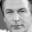
\includegraphics[scale = 0.19]{facescrub_actors_uncropped/Alec Baldwin22}
  \caption{Color image}\label{fcolor}
\endminipage\hfill
\minipage{0.32\textwidth}%
  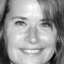
\includegraphics[scale = 0.17]{facescrub_actresses_uncropped/Lorraine Bracco34}
  \caption{image contain multiple actors}\label{fmulti}
\endminipage
\end{figure}

However, there are some images that are auto-generated due to dead URLs. Some examples are shown below:

\begin{figure}[!htb]
\minipage{0.32\textwidth}
  
\includegraphics[scale = 0.3]{facescrub_actors_uncropped/Bill Hader60}
  \caption{Dead URL1}\label{ferror1}
\endminipage\hfill
\minipage{0.32\textwidth}
  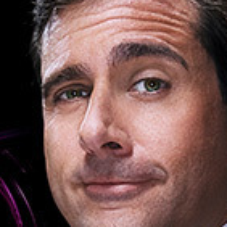
\includegraphics[scale = 0.13]{facescrub_actors_uncropped/Steve Carell92}
  \caption{Dead URL2}\label{ferror2}
\endminipage\hfill
\end{figure}

Most bounding box are accurate. The cropped-out faces do not necessarily align to each other as some are side face and some are frontal face. Some examples are shown below:

\begin{figure}[!htb]
\minipage{0.2\textwidth}
  
\includegraphics[scale = 2]{facescrub_actors_cropped/Bill Hader74}
  \caption{Side Face1}\label{sideface1}
\endminipage\hfill
\minipage{0.2\textwidth}
  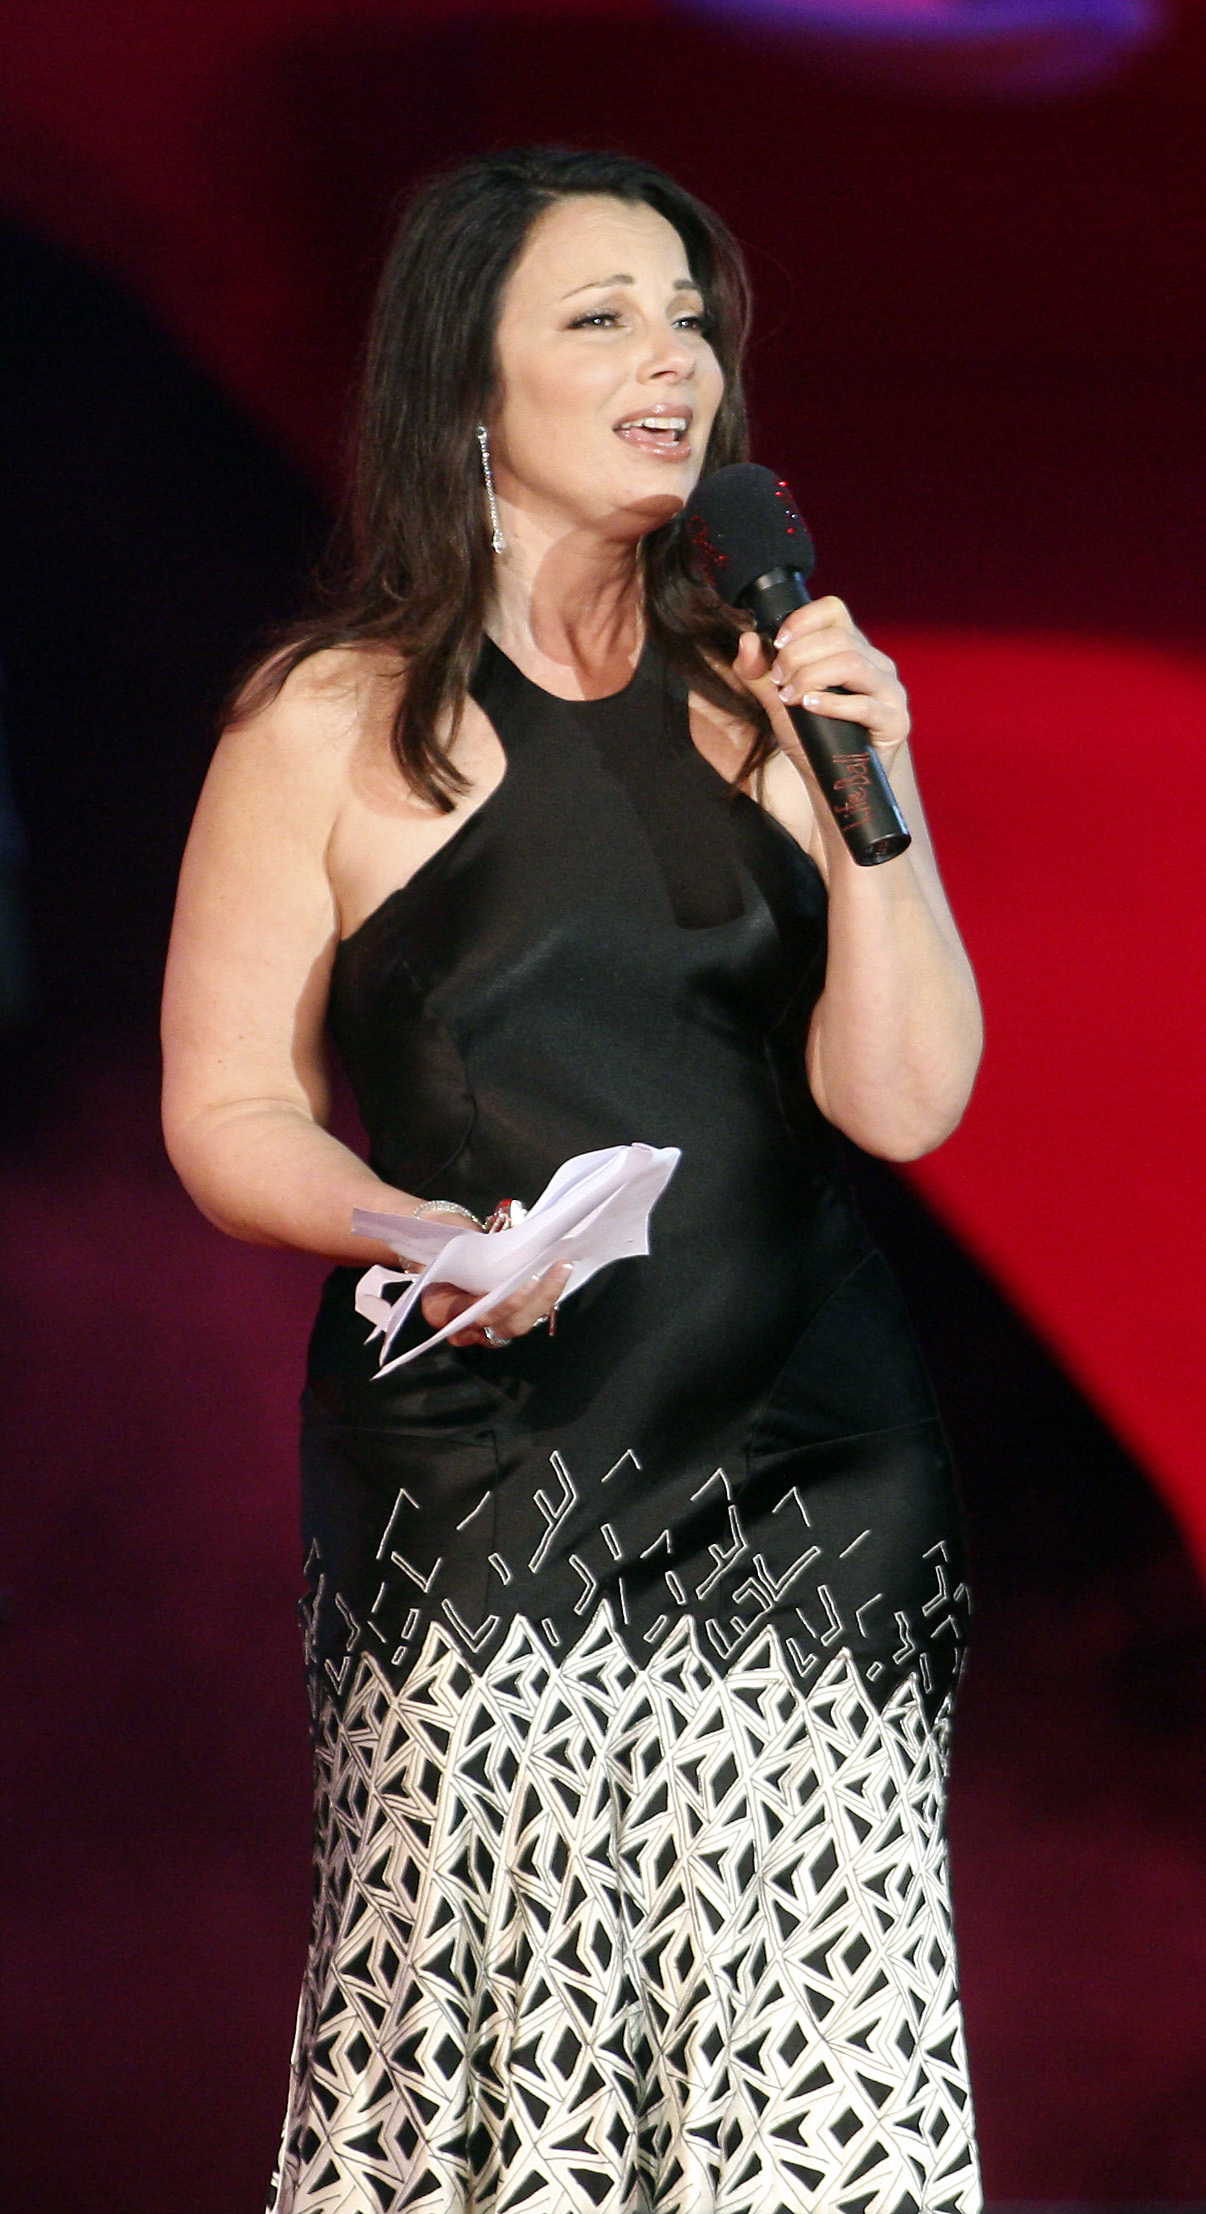
\includegraphics[scale = 2]{facescrub_actresses_cropped/Fran Drescher40}
  \caption{Side Face2}\label{sideface2}
\endminipage\hfill
\minipage{0.2\textwidth}
  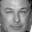
\includegraphics[scale = 2]{facescrub_actors_cropped/Alec Baldwin1}
  \caption{Frontal Face1}\label{frontface1}
\endminipage\hfill
\minipage{0.2\textwidth}
  
\includegraphics[scale = 2]{facescrub_actresses_cropped/Fran Drescher5}
  \caption{Frontal Face2}\label{frontface2}
\endminipage\hfill
\end{figure}

\newpage
However, few images' bounding box are incorrect. Those incorrect bounding box may cause disturbance on our training. Some examples are shown below:
\begin{figure}[!htb]
\minipage{0.5\textwidth}
  \includegraphics[scale = 0.5]{facescrub_actresses_uncropped/Fran Drescher102}
  \caption{uncropped image 1 with incorrect box}\label{wrongbox10}
\endminipage\hfill
\minipage{0.5\textwidth}
  \includegraphics[scale = 5]{facescrub_actresses_cropped/Fran Drescher102}
  \caption{cropped image 1 with incorrect box}\label{wrongbox11}
\endminipage\hfill
\end{figure}

\begin{figure}[!htb]
\minipage{0.5\textwidth}
  \includegraphics[scale = 0.5]{facescrub_actors_uncropped/Bill Hader95}
  \caption{uncropped image 2 with incorrect box}\label{frontface1}
\endminipage\hfill
\minipage{0.5\textwidth}
  \includegraphics[scale = 5]{facescrub_actors_cropped/Bill Hader95}
  \caption{cropped image 2 with incorrect box}\label{frontface2}
\endminipage\hfill
\end{figure}
\end{homeworkProblem}
\clearpage

%----------------------------------------------------------------------------------------
%	PROBLEM 2
%----------------------------------------------------------------------------------------

\begin{homeworkProblem}
\noindent \textit{Randomly Choose Training Sets, Validation Sets, and Test Sets}\\
The code for this part is defined as function $part2()$. This function return a dictionary named $act\_data$ whose keys are the actor's name, and the corresponding value is a list of array with length of 3, where the first element is a array that contains the training set, the second element is the array that contains the validation set and the third element is the array that contains the test set.\\

The function loads all the cropped images for each actor into a dictionary named $act\_rawdata$, and the dictionary has a following structure: the key is the actor's name and the corresponding value is a array that contains all the cropped images for that specific actor. Note that when loading the cropped images, the cropped images is flatten into a column vector. After loading the cropped images, it shuffles the columns of images array for each actors. For the sake of reproducibility, $numpy.random.seed()$ is implemented to shuffle the columns. Since there may be the cases where the total number of images available for one actor is less than 90, we let the the size of training data be $min(70, number of images avilable - 20)$. So for each actor, the corresponding training set which is stored in $act\_data[<actor's name>][0]$ contains the 0th to $min(70, number of images avilable - 20)$th columns of the shuffled array $act\_rawdata[<actor's name>]$. The validation set contains the -20th to -10th columns of the shuffled array, and the test set contains the -10th to the -1st columns of the shuffled array.\\

The code is pasted below.

\begin{lstlisting}
def part2(s = 0):
    act = ['Alec Baldwin', 'Bill Hader', 'Daniel Radcliffe', \
    'Gerard Butler', 'Michael Vartan', 'Steve Carell', \
    'America Ferrera', 'Angie Harmon', 'Fran Drescher', \
    'Kristin Chenoweth', 'Lorraine Bracco', 'Peri Gilpin']
    act_rawdata = {}
    act_data = {}
    for i in act:
        act_rawdata[i] = np.empty((1024,0))
        act_data[i] = [0, 0, 0]

    for j in ['actors', 'actresses']:
        act_type = j
        dataset_path = dirpath + "/facescrub_" + act_type + "_cropped/"
        for root, dirs, files in os.walk(dataset_path):
            dirs.sort()
            files.sort()
            for filename in files:
                im = imread(dataset_path + filename)
                im = im/255.
                im = np.array([im.flatten()]).T
                if np.amax(im) > 1.0 or np.amin(im) < 0. \
                or np.isnan(im).any() or np.isinf(im).any():
                    continue
                else:
                    for i in act:
                        if i in filename:
                            act_rawdata[i] = np.hstack((act_rawdata[i], im))

    # randomly shuffle act_rawdata
    np.random.seed(s)
    for i in act:
        act_rawdata[i] = act_rawdata[i][:,np.random.permutation\
        (act_rawdata[i].shape[1])]

    # act_data is a dictionary whose key is the name of actor/actress, value 
    #is the 3-element long array that the first
    # element is a array that contains the training set,
    # second one contains validation set, third one
    # contains test set.
    for i in act:
        act_data[i][0] = act_rawdata[i][:, :min(70, act_rawdata[i].shape[1] - 20)]
        act_data[i][1] = act_rawdata[i][:, -20:-10]
        act_data[i][2] = act_rawdata[i][:, -10:]
    return act_data

\end{lstlisting}

\end{homeworkProblem}
\clearpage

%----------------------------------------------------------------------------------------
%	PROBLEM 3
%----------------------------------------------------------------------------------------

\begin{homeworkProblem}
\noindent \textit{Linear Regression Classifier to distinguish Alec Baldwin and Steve Carell}\\
In this part, linear regression is used to classify whether a image is Alec Baldwin or Steve Carell. So quadratic loss is used as the cost function:
\begin{align*}
\sum_{i=1}^{m} (h_{\theta}(x^{(i)})-y^{(i)})^{2}
\end{align*}
The label of Alec Baldwin is set to 1 and the label of Steve Carell is set to -1. The prediction of images is obtained as:

\begin{itemize}
\item if hypothesis $h_{\theta}(x)$ is greater than 0, then predict $x$ having label of 1, which mean this image is Alec Baldwin in this case.
\item if hypothesis $h_{\theta}(x)$ is less than 0, then predict $x$ having label of -1, which mean this image is Steve Carell in this case.
\end{itemize}

The performance is reported by dividing the number of images being correctly classified by the number of total images being classified.\\

In order to get the linear regression to work, the learning rate $\alpha$ need to be no too large, otherwise the algorithm would not converge. However, too small learning rate will lead to slow convergence. Through the function $part3\_alpha()$, we can obtain the largest alpha that will lead to divergence. This function tries several different learning rates and plots cost function value vs. number of iterations with different learning rates. The result is shown below in Figure~\ref{31}. From the plot, alpha of 0.000021 leads to divergence. So selecting alpha as 0.00001 which is the largest number that will not lead to divergence to faster the gradient descent.
\begin{figure}[!htb]
\begin{center}
  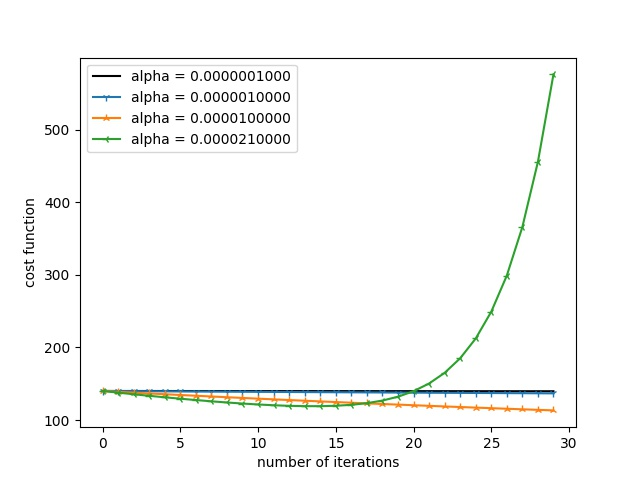
\includegraphics[scale = 0.4]{part3_1}
  \caption{cost function value vs. number of iterations with different learning rates}\label{31}
\end{center}
\end{figure}

With initial thetas being all zeros, learning rate $alpha$ being 0.00001, maximum number of iteration being 80000 which is chosen such that there is no early stop occurred, and stopping condition $EPS$ being 0.00001 which is given in the code provided in CSC411, the result is as following:\\ \\
This is the result for part3\\
('Cost function on training set:', 0.21649685023182624, 'Normalized:', 0.0015464060730844731)\\
('Cost function on validation set:', 18.09173743126312, 'Normalized:', 0.90458687156315598)\\
('Performance on training set', 1.0)\\
('Performance on validation set', 0.85)\\ 

The code used in this part is pasted below:\\
Note: $f$ is to calculate the cost function, $df$ is to calculate the gradient, $grad\_descent$ is to function for gradient descent. Those three functions is modified from the code provided in class. $performance$ is to calculate the performance of the theta in one particular dataset. $part3()$ consists of setting up training set, validation set, and test set, initializing theta, calling function $grad\_descent$ and calculating the performance.
\begin{lstlisting}
def f(x, y, theta):
    x = vstack((ones((1, x.shape[1])), x))
    return sum((y - dot(theta.T, x)) ** 2)


def df(x, y, theta):
    x = vstack((ones((1, x.shape[1])), x))
    return -2 * sum((y - dot(theta.T, x)) * x, 1)


def performance(X, Y, theta):
    X = vstack((np.ones((1, X.shape[1])), X))
    h = dot(theta.T, X)
    cor = 0
    for i in range(len(Y)):
        if Y[i] == 1 and h[i] > 0:
            cor += 1
        elif Y[i] == -1 and h[i] < 0:
            cor += 1
    return float(cor) / len(Y)


def grad_descent(f, df, x, y, init_t, alpha, EPS=1e-5, max_iter=80000):
    prev_t = init_t - 10 * EPS
    t = init_t.copy()
    iter = 0
    cost_func_ = []
    while norm(t - prev_t) > EPS and iter < max_iter:
        cost_func_.append(f(x,y,t))
        prev_t = t.copy()
        t -= alpha * df(x, y, t)
        if iter % 500 == 0:
            print "Iter", iter
            print "Cost", f(x, y, t)
            print "Gradient: ", df(x, y, t), "\n"
        iter += 1
        
    return t, cost_func_

def part3(alpha= 0.000010, st_devi = 0, max_iteration = 80000):
    X_train = np.hstack((act_data['Alec Baldwin'][0], act_data['Steve Carell'][0]))
    Y_train = np.append(np.ones(act_data['Alec Baldwin'][0].shape[1]),
                        np.full(act_data['Steve Carell'][0].shape[1], -1))
    X_vali = np.hstack((act_data['Alec Baldwin'][1], act_data['Steve Carell'][1]))
    Y_vali = np.append(np.ones(10), np.full(10, -1))
    X_test = np.hstack((act_data['Alec Baldwin'][2], act_data['Steve Carell'][2]))
    Y_test = np.append(np.ones(10), np.full(10, -1))

    np.random.seed(0)
    theta0 = np.random.normal(scale=st_devi, size=1025)
    theta, cost_func_ = grad_descent(f, df, X_train, Y_train, \
    theta0, alpha, max_iter = max_iteration)

    print("This is the result for part3")
    print("Cost function on training set:", f(X_train, Y_train, theta),\
     "Normalized:", f(X_train, Y_train, theta)/(Y_train.shape[0]))
    print("Cost function on validation set:", f(X_vali, Y_vali, theta),\
     "Normalized:", f(X_vali, Y_vali, theta)/(Y_vali.shape[0]))
    print("Performance on training set", performance(X_train, Y_train, theta))
    print("Performance on validation set", performance(X_vali, Y_vali, theta))

    return theta

def part3_alpha():
    X_train = np.hstack((act_data['Alec Baldwin'][0], act_data['Steve Carell'][0]))
    Y_train = np.append(np.ones(act_data['Alec Baldwin'][0].shape[1]),
                        np.full(act_data['Steve Carell'][0].shape[1], -1))
    X_vali = np.hstack((act_data['Alec Baldwin'][1], act_data['Steve Carell'][1]))
    Y_vali = np.append(np.ones(10), np.full(10, -1))
    X_test = np.hstack((act_data['Alec Baldwin'][2], act_data['Steve Carell'][2]))
    Y_test = np.append(np.ones(10), np.full(10, -1))

    fig = plt.figure(31)
    alpha_ = [1e-7, 1e-6, 1e-5, 2.1e-5]
    for j, i in zip(range(len(alpha_)), alpha_):
        np.random.seed(0)
        theta0 = np.random.normal(scale=0, size=1025)
        theta, cost_func_ = grad_descent(f, df, X_train, Y_train,\
         theta0, i, max_iter = 30)
        plt.plot(range(0,30), cost_func_, "-%i"%j, label = "alpha = %010.10f"%i)
    plt.xlabel("number of iterations")
    plt.ylabel('cost function')
    plt.legend(loc = "best")

    fig.savefig(dirpath + '/part3_1.jpg')
    plt.show()
    return
\end{lstlisting} 
\end{homeworkProblem}
\clearpage
%----------------------------------------------------------------------------------------
% 	PROBLEM 4
%----------------------------------------------------------------------------------------
\begin{homeworkProblem}
\noindent \textit{Display Theta}

\subsubsection*{a)}
The figures shown below are generated by calling the function $part4a()$. This function removes the off-set $\theta_{0}$ and resizes the theta back to 32$\times$32. The left figure shows the thetas obtained by using the full training set, the right figure shows the thetas obtained by using only two images of each actors. From the figures, two images of each actor results a obvious face, which indicates that the theta obtained refers to some specific images of the actors. On the other hands, the visualization  of the thetas obtained by using full training set does not have any obvious face, which indicates that it is more "generalized" than that obtained by using two images of each actors.  So the thetas obtained by using the full training set should perform better on validation and test sets.
\begin{figure}[!htb]
\begin{center}
  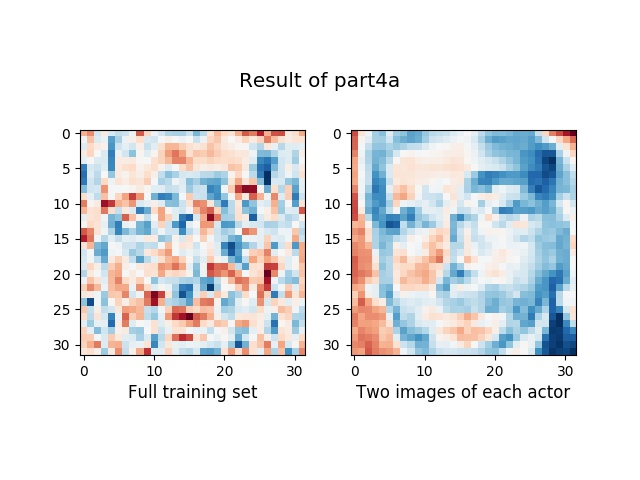
\includegraphics[scale = 0.8]{result_of_part4a}
  \caption{result of part4a)}\label{4a}
\end{center}
\end{figure}

\subsubsection*{b)}

Note: The images in this section show the theta generated by initializing thetas by drawing it from a normal distribution with mean of 0 and standard deviation of std\_deviation (stated in the title of each image), and the maximum iteration being max\_itera (stated in the title of each image).\\

In order to generate a face-like image, we need to initialize theta closed to all zeros and set the maximum iteration to be small. In this case, the initial thetas are closed to the optimal point and early stop occurs. However, if the initial thetas are not closed to zeros and early stop occurs, the image of thetas does not contain any obvious images. Figure~\ref{41} shows the image with obvious face and Figure~\ref{42} shows the image without obvious face.\\

\begin{figure}[!htb]
\minipage{0.5\textwidth}
  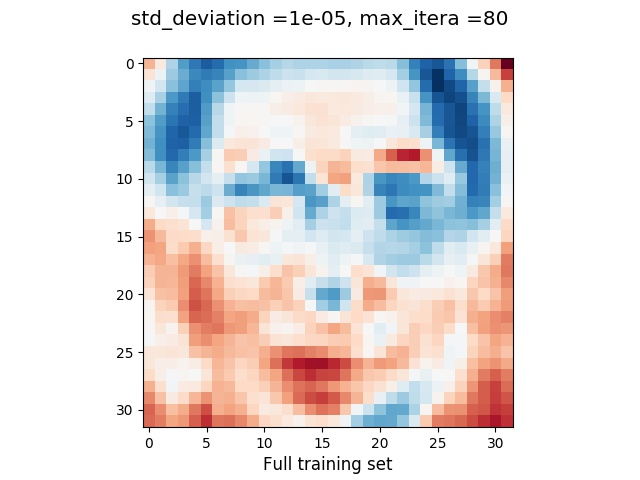
\includegraphics[scale = 0.37]{part4b_std_dev_1e-05_max_itera_80_}
  \caption{image with obvious face}\label{41}
\endminipage\hfill
\minipage{0.5\textwidth}
  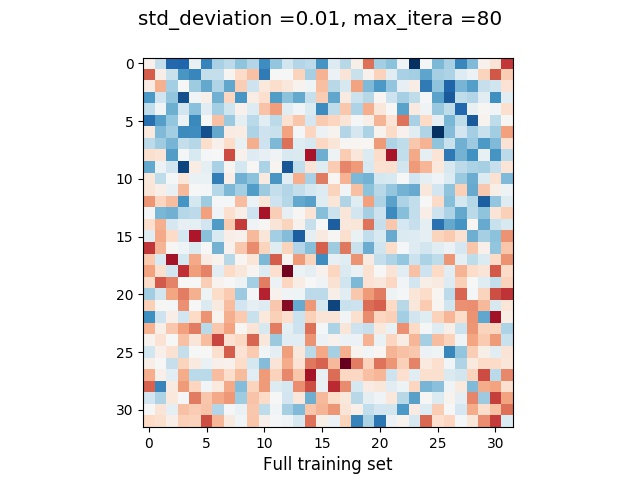
\includegraphics[scale = 0.37]{part4b_std_dev_0.01_max_itera_80_}
  \caption{image without obvious face}\label{42}
\endminipage\hfill
\end{figure}

To obtain back the left figure in Figure~\ref{4a}, no matter what initial theta is, as long as early stop does not occur and learning rate is small such that the algorithm converges, because the cost function, in this case, is a convex function. Convex function indicates that the local minimum is the global minimum. The images of theta generated by different initial thetas are shown below:
\begin{figure}[!htb]
\minipage{0.3\textwidth}
  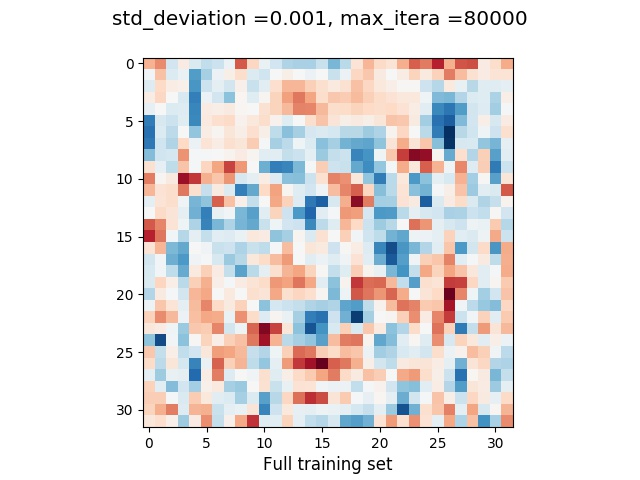
\includegraphics[scale = 0.28]{part4b_std_dev_0.001_max_itera_80000_}
  \caption{}\label{43}
\endminipage\hfill
\minipage{0.3\textwidth}
  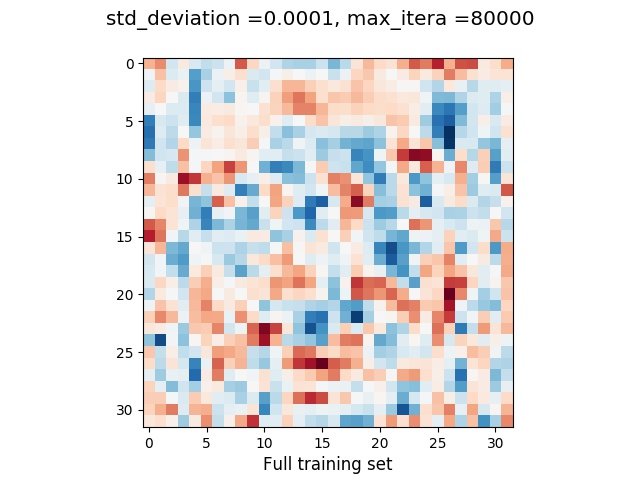
\includegraphics[scale = 0.28]{part4b_std_dev_0.0001_max_itera_80000_}
  \caption{}\label{44}
\endminipage\hfill
\minipage{0.3\textwidth}
  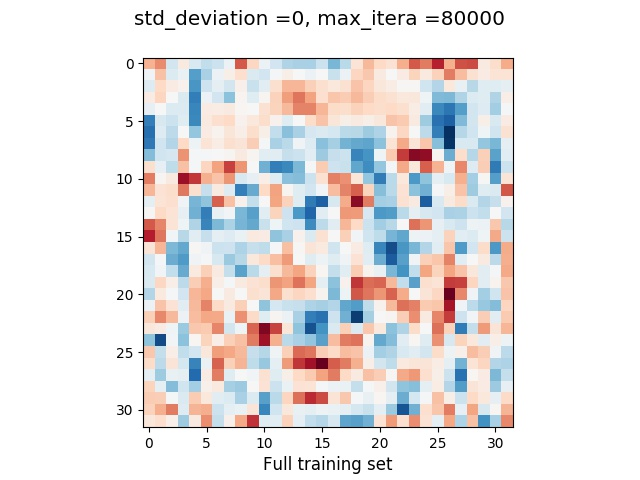
\includegraphics[scale = 0.28]{part4b_std_dev_0_max_itera_80000_}
  \caption{}\label{45}
\endminipage\hfill
\end{figure}
\end{homeworkProblem}
\clearpage


%----------------------------------------------------------------------------------------
% 	PROBLEM 5
%----------------------------------------------------------------------------------------
\begin{homeworkProblem}
\noindent \textit{Classify Gender}

In this question, we need to investigate how the size of the training affects the performance on the training and validation sets for the 6 actors in $act$ and on the validation sets for the 6 actors who are not in $act$. The size of training set ranges from 10\% to 100\% of the full training set. The parameter used in this problem such as learning rate, initial theta value, etc., are the same as those parameters used in part3. The plot of the performance on the training and validation sets for the 6 actors in $act$, and on the validation sets for the 6 actors who are not in $act$ vs. the size of the training set is shown below.

\begin{figure}[!htb]
\begin{center}
  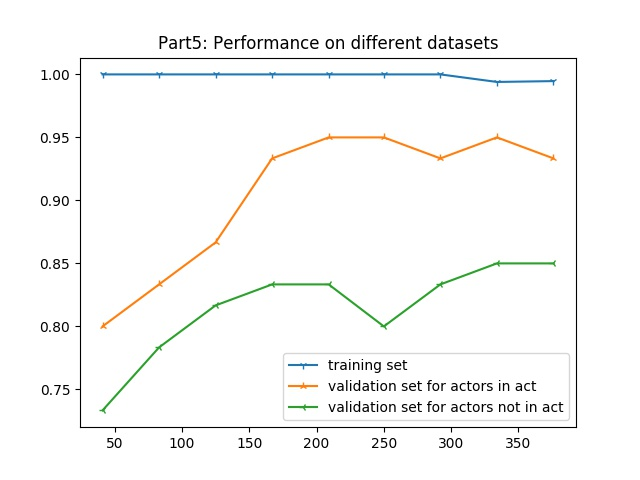
\includegraphics[scale = 0.7]{result_of_part5}
  \caption{}\label{5}
\end{center}
\end{figure}

The result shows that the performance on training set remains really high (about 100\%), although the performance slightly decrease as the size of the training set increases. The performance on the validation set of the acts who are in $act$ is always higher than that of the acts who are not in $act$. Performance on the validation of both the actors who are in $act$ and who are not in $act$ increases as the size of the training set increases. When the size of training set is small, overfitting problem occurs: performance on training set is much higher than the performance on both validation sets. As the size of training set increases, the difference between the performances on training set and validation sets decreases, which indicates it is less overfitting.
\end{homeworkProblem}


%----------------------------------------------------------------------------------------
% 	PROBLEM 6
%----------------------------------------------------------------------------------------
\begin{homeworkProblem}
\subsubsection*{a)}
\noindent \textit{Compute $\frac{\partial J}{\partial \theta_{pq}}$}\\
\iffalse
The cost function is:
\begin{align*}
J(\theta) = \sum^{m}_{i=1}{(\sum^{k}_{j=1}{(\theta^{T}x^{(i)}-y^{(i)})^{2}_{j}})}
\end{align*}
So the partial derivative of the cost function is:
\begin{align}
\frac{\partial J}{\partial \theta_{pq}} &= \frac{\partial }{\partial \theta_{pq}}\bigg[\sum^{m}_{i=1}{(\sum^{k}_{j=1}{(\theta^{T}x^{(i)}-y^{(i)})^{2}_{j}})}\bigg] \nb\\
&= \sum^{m}_{i=1}{\frac{\partial }{\partial \theta_{pq}}\bigg[(\sum^{k}_{j=1}{(\theta^{T}x^{(i)}-y^{(i)})^{2}_{j}})\bigg]} \nb \\
&= \sum^{m}_{i=1}{\frac{\partial }{\partial \theta_{pq}}\bigg[(\theta^{T}x^{(i)}-y^{(i)})^{2}_{1}+(\theta^{T}x^{(i)}-y^{(i)})^{2}_{2} + ... + (\theta^{T}x^{(i)}-y^{(i)})^{2}_{q} + ...+ (\theta^{T}x^{(i)}-y^{(i)})^{2}_{k}\bigg]}\\
&= \sum^{m}_{i=1}{\frac{\partial }{\partial \theta_{pq}}(\theta^{T}x^{(i)}-y^{(i)})^{2}_{q}}\\
&= \sum^{m}_{i=1}{\bigg[2\cdot \Big(\frac{\partial }{\partial \theta_{pq}}(\theta^{T}_{q}x^{(i)})\Big)\cdot (\theta^{T}x^{(i)}-y^{(i)})_{q}\bigg]}
\end{align}

\begin{align}
\frac{\partial }{\partial \theta_{pq}}(\theta^{T}_{q}x^{(i)}) &= \frac{\partial }{\partial \theta_{pq}}\bigg[\sum^{n}_{l=1}{\theta^{T}_{ql}x^{(i)}_{l}}\bigg] \nonumber \\
&= 
\end{align}
\fi
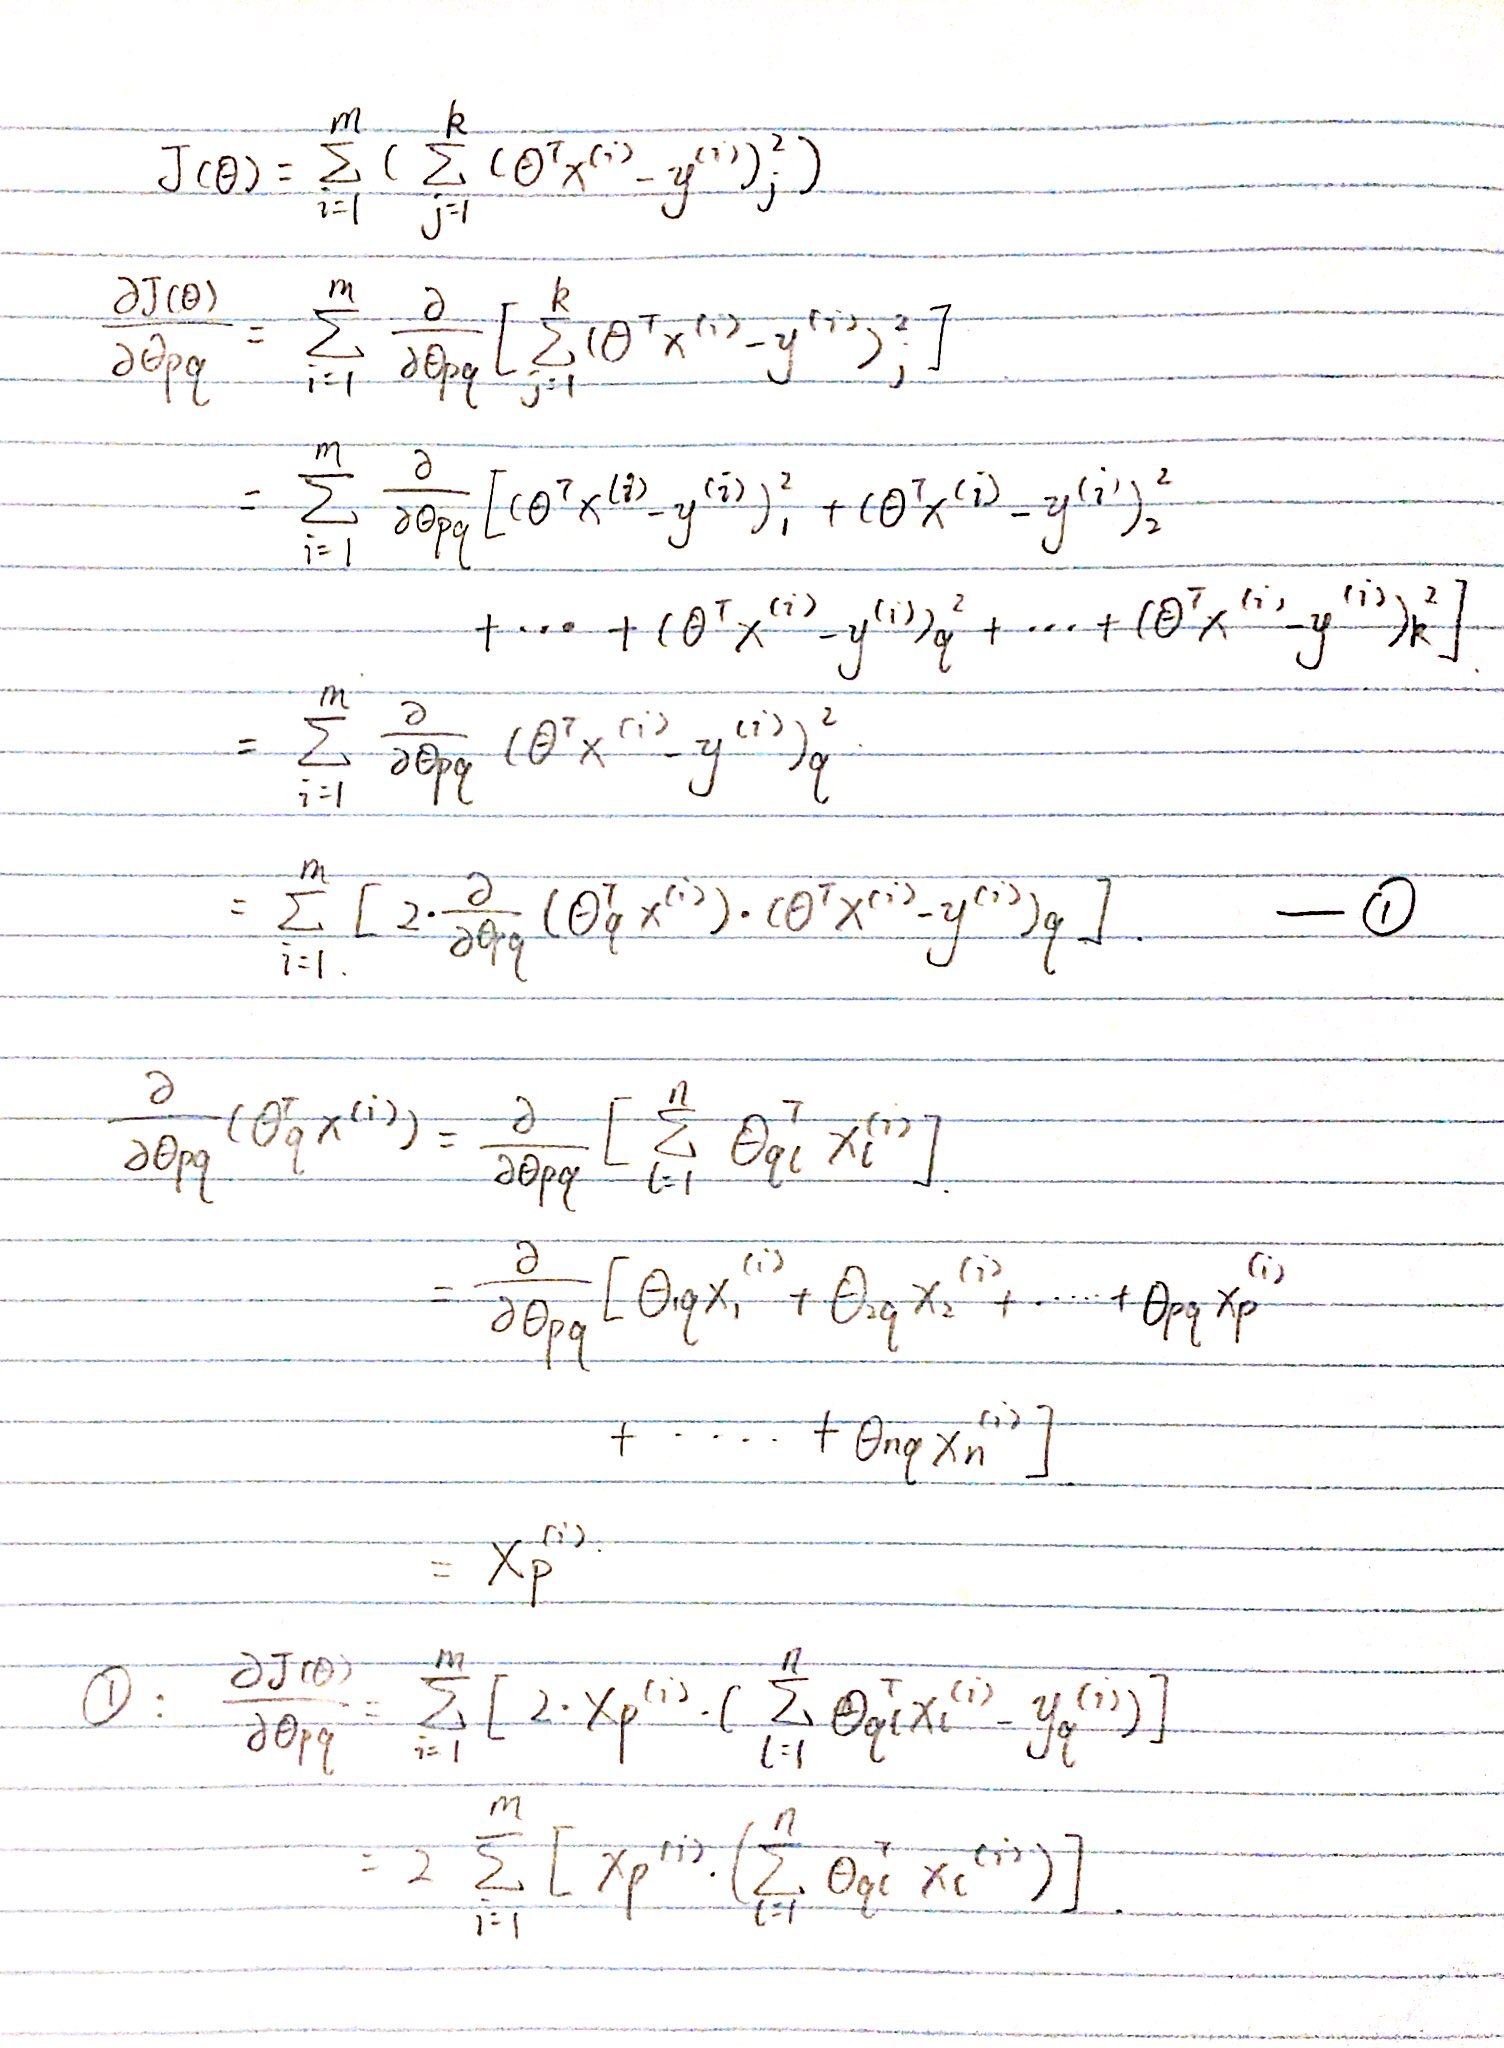
\includegraphics[scale=0.3]{6a}
\subsubsection*{b)}
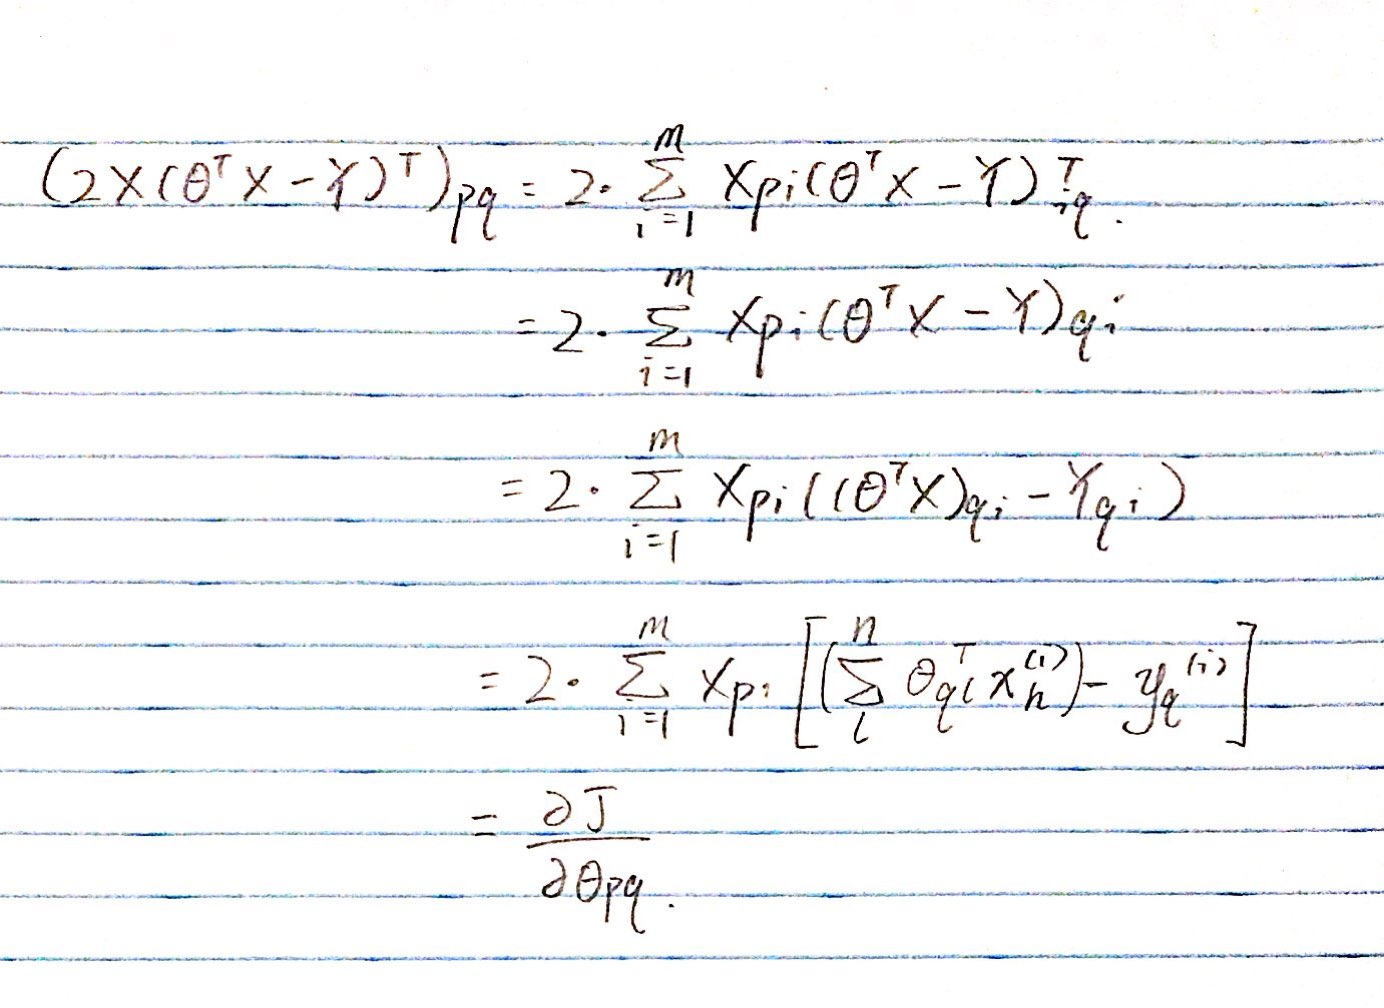
\includegraphics[scale=0.3]{6b}
\clearpage
\subsubsection*{c)}
$f\_multi$ is a modified function to calculate the cost function, $df\_multi$ is a modified function to calculate the gradient. 
\begin{lstlisting}
def f_multi(x, y, theta):
    x = vstack( (ones((1, x.shape[1])), x))
    return np.sum( (y - dot(theta.T,x)) ** 2)

def df_multi(x, y, theta):
    x = vstack( (ones((1, x.shape[1])), x))
    return 2 * dot(x, (dot(theta.T,x) - y).T)
\end{lstlisting}
 

\clearpage
\subsubsection*{d)}
Comparison between gradient obtained by vectorized gradient function and gradient obtained by finite-difference approximations is used to verify that the vectorized gradient function stated in part 6c works properly. The finite-difference approximation is given below:

\begin{align*}
\frac{\partial f}{\partial \theta_{i}} \approx \frac{f(\theta_{1}, \theta_{2}, ..., \theta_{i}+h, ..., \theta_{n}) - f(\theta_{1}, \theta_{2}, ..., \theta_{i}, ..., \theta_{n})}{h}
\end{align*}

In this case, the $f$ is the cost function which is calculated by function $f\_multi$ and the variable is $theta$. The training set contains all the images in training sets($act\_data$[actor's name]$[0]$ obtained at part2) for all actors in $act$. The verification initializes the theta to be all zeros, run 50 iterations of gradient descent, then calculate the gradient obtained by vectorized gradient function(through function $df\_multi$) and by finite-difference approximations(through function $finite\_diff$). The selection of h is quite critical because mathematically, smaller h leads to more accuracy approximation; however, too small h will lead to underflow problem when using computer, which can significantly increases inaccuracy. So in order to select the optimal h, I calculated the average difference over 5 coordinates with different h. A plot of average difference over 5 coordinates vs. h is shown below.

\begin{figure}[!htb]
\begin{center}
  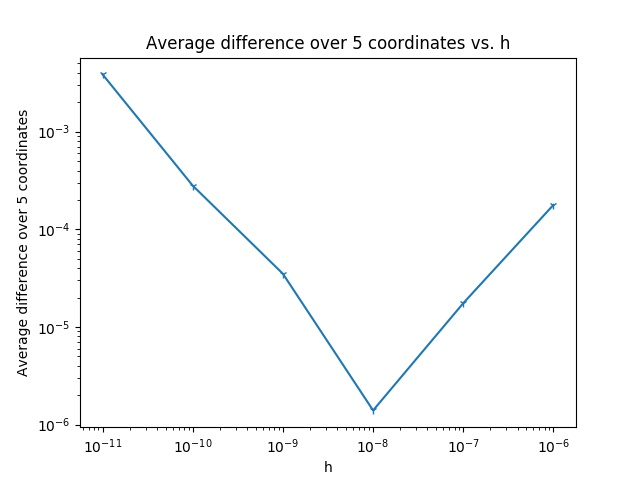
\includegraphics[scale = 0.4]{part6d_1}
  \caption{}\label{6}
\end{center}
\end{figure}

As shown in the figure, selecting h as $10^{-8}$ gives us a accurate approximation. The difference along 5 coordinates with h as $10^{-8}$ are:\\
Difference in gradient[235, 0] is 0.0000018104\\
Difference in gradient[905, 1] is 0.0000017559\\
Difference in gradient[715, 4] is 0.0000013999\\
Difference in gradient[847, 5] is 0.0000009059\\
Difference in gradient[960, 4] is 0.0000011250\\

The code used in this part is pasted below:
\begin{lstlisting}
def finite_diff(f, x, y, theta, row, col, h):
    #function for calculating one component of gradient 
    #using finite-difference approximation
    theta_h = np.copy(theta)
    theta_h[row,col] = theta_h[row,col] + h
    return (f(x, y ,theta_h) - f(x, y, theta))/h
    
def part6d():
    #construct training set
    act1 = ['Lorraine Bracco', 'Peri Gilpin', 'Angie Harmon', 'Alec Baldwin', \
    'Bill Hader', 'Steve Carell']

    X_train = np.empty((1024, 0))
    Y_train = np.empty((len(act1), 0))
    for i in range(len(act1)):
        temp = np.zeros((len(act1), act_data[act1[i]][0].shape[1]))
        temp[i, :] = 1
        X_train = np.hstack((X_train, act_data[act1[i]][0]))
        Y_train = np.hstack((Y_train, temp))

    #run 50 iterations of gradient descent
    np.random.seed(1)
    theta0 = np.random.normal(scale=0, size=(1025, 6))
    theta, cost_func_ = grad_descent(f_multi, df_multi, X_train, Y_train, \
    theta0, 0.000001, max_iter=50)
    gradient = df_multi(X_train, Y_train, theta)
    
    #pick 5 random coordinates
    np.random.seed(1)
    row_ = np.random.randint(0,1026,5)
    col_ = np.random.randint(0,7,5)
    h_ = (10**exp for exp in range(-11,-5))
    error_ = []
    hh =  []
    for h in h_:
        hh.append(h)
        temp = 0
        for i in range(5):
            temp += abs(finite_diff(f_multi, X_train, Y_train, theta, row_[i],\
                                    col_[i],h) - gradient[row_[i], col_[i]])
        error_.append(temp/5.)
    
    #save figure
    fig = plt.figure(6)
    plt.title('Average difference over 5 coordinates vs. h')
    plt.xlabel('h')
    plt.ylabel("Average difference over 5 coordinates")
    plt.loglog(hh,error_,'-1')

    fig.savefig(dirpath + '/part6d_1.jpg')
    plt.show()

    #print out result
    for i in range(5):
        print("Difference in gradient[%i, %i] is %010.10f" %(row_[i], col_[i] \
              ,abs(finite_diff(f_multi, X_train, Y_train, theta, row_[i],\
                                col_[i],10**(-8)) - gradient[row_[i], col_[i]])))
         
    return
\end{lstlisting}
\end{homeworkProblem}
\clearpage
%----------------------------------------------------------------------------------------
% 	PROBLEM 7
%----------------------------------------------------------------------------------------
\begin{homeworkProblem}
\noindent \textit{Face Recognition on Six Actors}\\
$h_{\theta}(x)$ in this part is a vector and the original label is a vector that only one element being 1 and other elements are zeros. So we need to transform our prediction in the same format as the original label: the maximum value among $h_{\theta}(x)$ is considered as 1 and other values are considered as 0. For example, say $h_{\theta}(x)$ is [0.1,0.7,0.3,0.5,0.1,0.4]; then, the transformed prediction is [0,1,0,0,0,0].\\

In this part, we need to tune parameters in order to get this algorithm functions properly. Similar to part3, we initialize thetas to be all zeros. The selection of learning rate is done in the same fashion as how it is chosen in part3. The result (can be obtained by calling function $part7_alpha()$) is shown below in Figure~\ref{71}. From the plot, alpha of 0.0000072 leads to divergence. So selecting alpha as 0.000004 which is the largest number that will not lead to divergence to faster the gradient descent.\\

\begin{figure}[!htb]
\begin{center}
  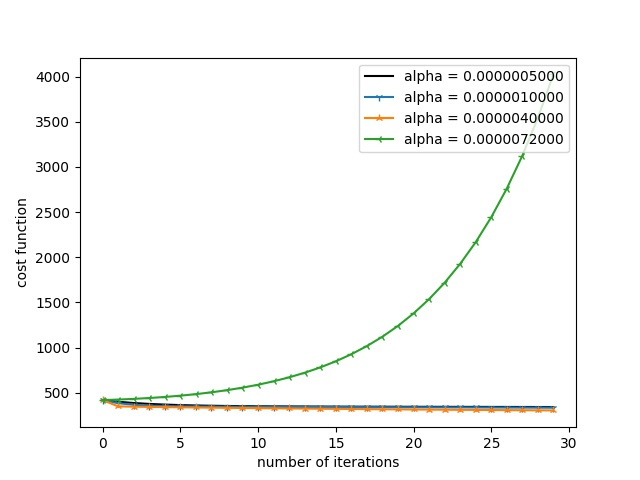
\includegraphics[scale = 0.5]{part7_1}
  \caption{}\label{71}
\end{center}
\end{figure}

We also need to tune maximum number of iteration as overfitting might occur in this problem. So the gradient descent should stop when the it has best performance on validation set rather than at time when the cost function is minimized. A plot shown (can be obtained by calling function $part7_itera()$)in Figure~\ref{72} below shows the relation between the maximum number of iterations and the performance on the validation set. From the figure, the model performs the best on validation set when maximum number of iterations is around 10000.\\

\clearpage
\begin{figure}[!htb]
\begin{center}
  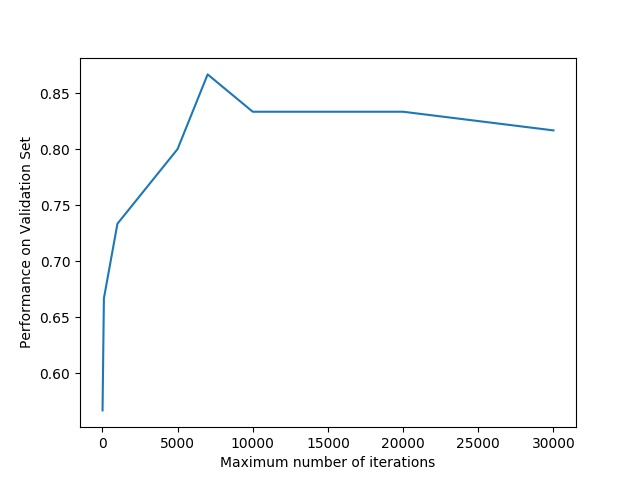
\includegraphics[scale = 0.5]{part7_2}
  \caption{}\label{72}
\end{center}
\end{figure}

With initial thetas being all zeros, learning rate $alpha$ being 0.000004, maximum number of iteration being 10000,  and stopping condition $EPS$ being 0.00001 which is given in the code provided in CSC411, the result is as following:\\

this is the result for part7\\
('Cost function on training set:', 74.955443686355764, 'Normalized:', 12.49257394772596)\\
('Cost function on validation set:', 22.737504560791393, 'Normalized:', 3.7895840934652321)\\
('Cost function on validation set:', 29.54362318656392, 'Normalized:', 4.9239371977606536)\\
('Performance on training set', 0.9832535885167464)\\
('Performance on validation set', 0.8333333333333334)\\
('Performance on test set', 0.8333333333333334)\\
\end{homeworkProblem}
\clearpage

%----------------------------------------------------------------------------------------
% 	PROBLEM 8
%----------------------------------------------------------------------------------------
\begin{homeworkProblem}
\noindent \textit{Visualization of thetas}
\begin{figure}[!htb]
\minipage{0.32\textwidth}
  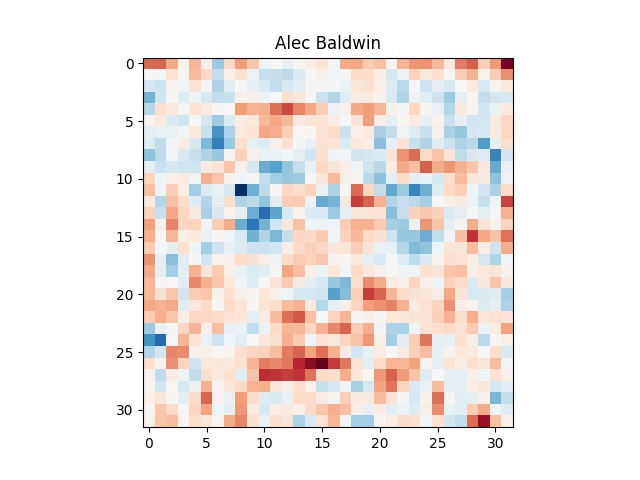
\includegraphics[scale = 0.27]{theta_for_Alec Baldwin}
  \caption{Alec Baldwin}
\endminipage\hfill
\minipage{0.32\textwidth}
  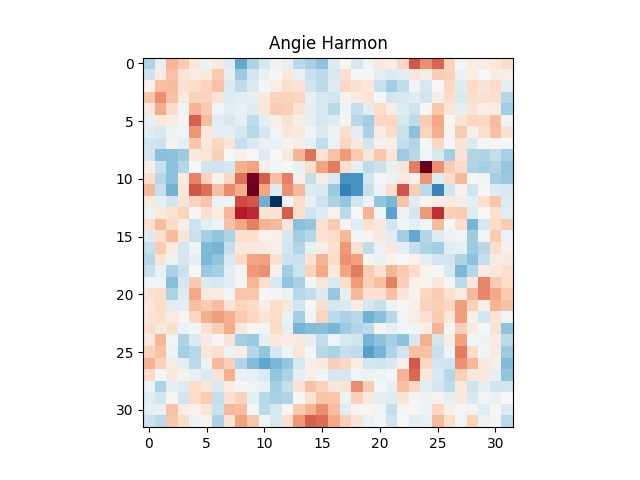
\includegraphics[scale = 0.27]{theta_for_Angie Harmon}
  \caption{Angie Harmon}
\endminipage\hfill
\minipage{0.32\textwidth}%
  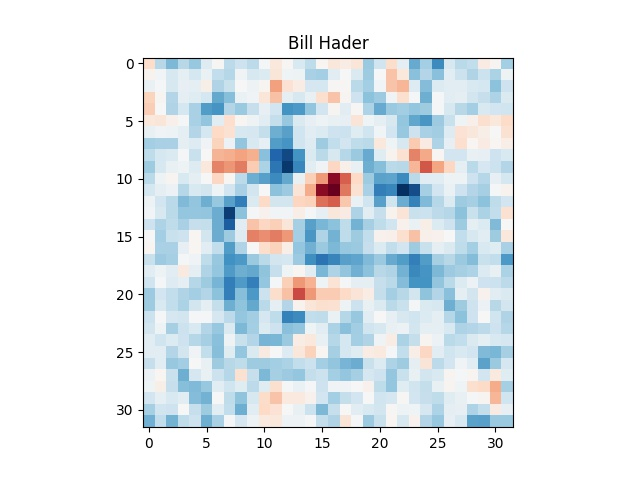
\includegraphics[scale = 0.27]{theta_for_Bill Hader}
  \caption{Bill Hader}
\endminipage
\end{figure}

\begin{figure}[!htb]
\minipage{0.32\textwidth}
  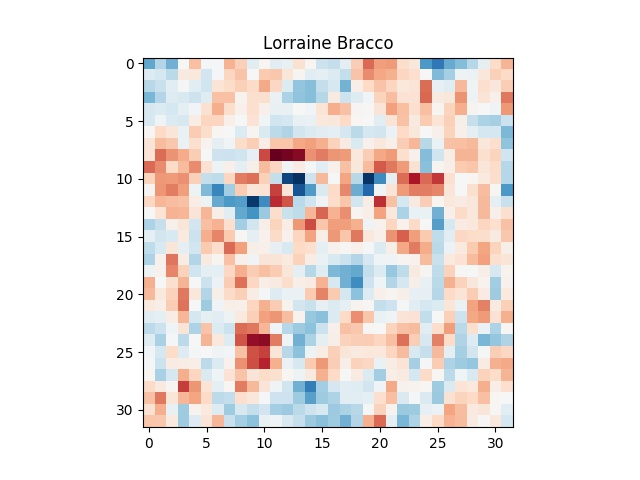
\includegraphics[scale = 0.27]{theta_for_Lorraine Bracco}
  \caption{Lorraine Bracco}\label{Lorraine Bracco}
\endminipage\hfill
\minipage{0.32\textwidth}
  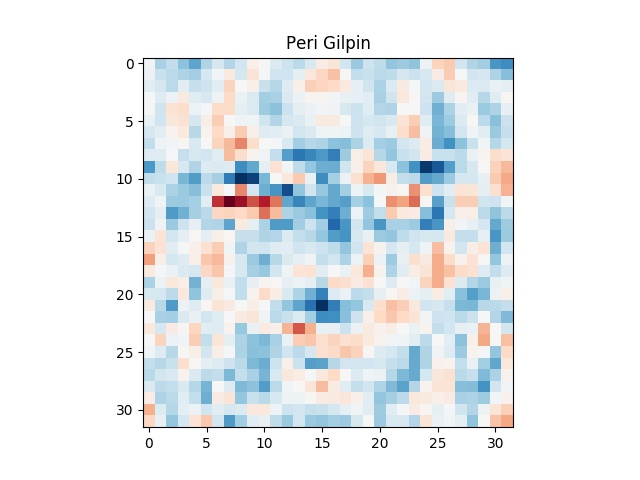
\includegraphics[scale = 0.27]{theta_for_Peri Gilpin}
  \caption{Peri Gilpin}\label{Peri Gilpin}
\endminipage\hfill
\minipage{0.32\textwidth}%
  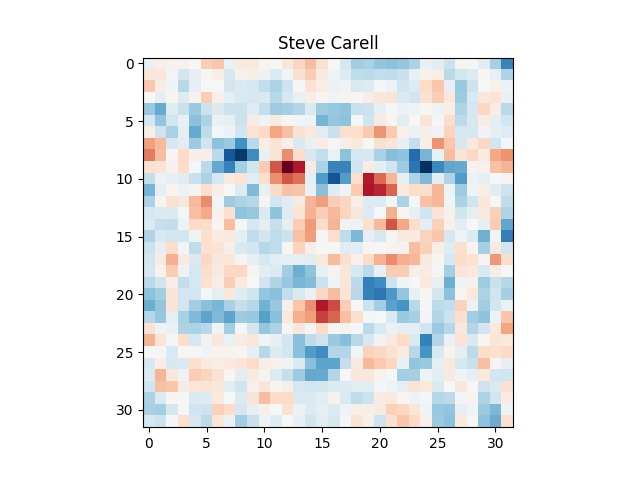
\includegraphics[scale = 0.27]{theta_for_Steve Carell}
  \caption{Steve Carells}\label{Steve Carell}
\endminipage
\end{figure}

\end{homeworkProblem}
\clearpage


\end{document}